\documentclass{article}
\usepackage{graphicx}
\usepackage{amsmath}
\usepackage{subfig}
\usepackage{float}
\usepackage{caption}
\usepackage[legalpaper, portrait, margin=1in]{geometry}

\title{Analysis of Hydride Structures in Micrographs of Zirconium Samples using Image Processing in Python}
\author{Group 1: S. Khan, A. Hanson, J. Larkin}
\begin{document}
	\maketitle
	
	\begin{center} \textit{This report details progress made during the Research Software \& Engineering in Python module, in which image processing techniques are utilised to automatically analyse micrograph images of zirconium hydride (H\textsubscript{4}Zr) structures in samples of metallic zirconium. Explanation of the method, including relevant images and discussion of code elements are included.} \end{center}
	
	\section{Introduction \& Review of Existing Literature}
	\subsection{Background}
	During the service lifetime of zirconium fuel cladding within a light-water reactor core, several phenomena manifest as a result of both direct neutron irradiation and chemical reactivity with the core coolant. One of the more prominent of these is the formation of zirconium hydride within the bulk material, resulting from the radiolysis of core coolant and subsequent migration of hydrogen through the lattice, which then reacts with the metal and accumulates at grain boundaries. As zirconium hydride is typically more brittle than the lattice itself, this serves to compromise the local integrity of the lattice. 
	\\
	\\
	Zirconium, as a HCP lattice, exhibits a specific crystal \textit{texture} which is determined during component fabrication, the result of which is the alignment of the $<0002>$ basal planes tangentially around the cladding tube. As hydrides typically accumulate parallel to the basal plane, this is advantageous as it prevents the development of cracks radially through the structure which can result in through-wall cracking, compromising the barrier between nuclear fuel and core coolant. Larger scale cracks are able to form due to the close proximity of hydride structures, permitting a brittle fracture through one hydride region to migrate to a neighbouring region, continuing until a large macroscopic crack manifests. This is herein referred to as \textit{hydride connectivity}.
	\\
	\\
	One beneficial technique for analysing these phenomena is the use of transmission electron microscopy (TEM), which generates two-dimensional micrographs of a thin sample slice and highlights changes in the sample composition, including the presence of hydride zones in a metallic matrix (see Figure~\ref{fig:tem_hydride_eg}). It is not known what microscopy technique was used to produce the hydride images in this study, however due to the low resolution of the images and the size of the hydrides it is thought to be TEM.
	\\
	\begin{figure}[h]
		\centering
		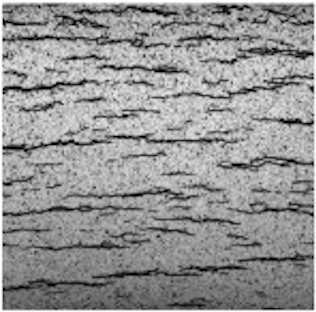
\includegraphics[width=2.5in]{Figures/tem_hydride_eg} 
		\caption{Typical TEM micrograph image of darker hydride bands within a zirconium matrix. The horizontal regions are sporadically connected together by small fractures within the material.}
		\label{fig:tem_hydride_eg}
	\end{figure}
	\\
	These micrographs may be processed using appropriate software environments to identify characteristics such as the density of hydride regions within the material, and the level to which connectivity is observed. Here, image processing techniques within the python programming environment are used to identify these properties, chiefly incorporating the \textit{scikit-image} series of algorithms along with originally-developed scripts. For this project, code is developed, implemented and tested to determine the most effective means of isolating and analysing hydride structures within the images. An account of the evolution of the techniques is given, and results are presented and discussed.
	\\
	\subsection{Literature Review}
	The degredation mechanics of zirconium alloys remain under review as the nuclear sector continues to improve the efficiency and safety of modern nuclear reactors. Research into the degradation of zirconium is a vital component of this research and as such there exists an extensive array of techniques under investigation for accurately predicting this degradation. Practical methods such as x-ray diffraction and resistivity assays are commonplace, however advances in computing power are placing an increased emphasis on the use of computer processing in both independent modelling and comparison with real-world observations.
	\\
	Image processing techniques are utilised for a wide array of different purposes owing to their versatility, reprogrammability and ease of automation. For samples such as micrographs which may exhibit minor differences between images, it is advantageous to automate the process of detecting characteristics to ensure all images are processed identically, therefore reducing systematic errors. In the context of zirconium analysis, several studies have aimed to predict failure routes and lifetime behaviour by quantifying the level and severity of microstructural damage caused by hydride plates evident within sample micrographs, achieved using a range of software packages.
	\\
	\\
	P.A. Simon et al. (2021) \cite{Simon2021} have recently analysed the link between \textit{radial} hydride structures in zirconium and likelihood of eventual failure in MATLAB, and quantified results using a figure known as the \textit{radial hydride continuous path} (RHCP), which considers the geometries of hydride plates, separation distances and the probability of crack propagation through the plates (for which individual regions are assigned a weighting factor). Here, a series of algorithms were used to find the 'best path' for which crack propagation between hydrides is most likely, with micrographs exhibiting more severe crack routes (of greater total length and probability of occurrence) generating a larger value for RHCP (between 0 and 1). The study utilised micrographs of real zirconium samples, binarised and 'cleaned' to remove noise from dust and imperfections within the matrix. It is noted that the complexity of real material micrographs can present issues for many algorithms and as such techniques such as splitting the image into smaller 'bands' are sometimes necessary. The study observed that for higher values of RHCP and r\textit{radial hydride fraction} (RHF), in which greater quantities of radial hydride plates and more crack routes are present, the \textit{fracture energy}, that is, the energy input required for a total fracture to manifest, decreased substantially.
	\\
	RHF as a similar metric to RHCP is used within this study with the similar goal of developing a foundation for predicting the failure modes within zirconium components.
	\\
	\begin{figure}[h]
		\centering
		\subfloat[The crack route through a cladding sample is less 'direct' through the material, as migration between hydride plates is more difficult.]{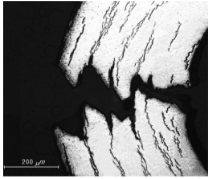
\includegraphics[width=0.45\textwidth]{Figures/circ_frac.PNG}\label{fig:circ_fract}}
		\hfill
		\subfloat[Here, several direct crack routes can be ween in the material owing to a large quantity of radial hydrides, presenting significantly increased probability of through-wall cracking.]{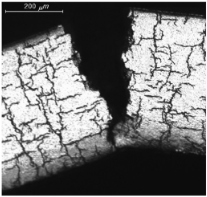
\includegraphics[width=0.4\textwidth]{Figures/rad_frac.PNG}\label{fig:rad_fract}}
		\caption{Micrographs of sections of cladding with varying hydride morphologies. The fracture route aligns more directly through the material for (b), in which a greater quantity of radially-oriented hydrides are observed. (a) exhibits more circumferentially-aligned hydrides which make crack propagation more difficult.}
		\label{fig:rad_circ_frac}
	\end{figure}
	\\
    Similarly, the fracture morphologies in oxidised samples of Zircaloy-4 have been investigated by P.A. Raynaud et al. (2012) \cite{RAYNAUD201269}.
	\\
	\section{Initial Image Processing}
	\subsection{The Gaussian Blur}
	To begin this project, a series of pre-prepared micrograph images were manipulated and several different approaches in python were tested to provide an initial understanding of the basics of image processing. Algorithms were written which could apply different threshold filters to image value arrays once they had been read into python. When the images were read by the \textit{Scikit image} package in python, they could be expressed as a numerical array with \textit{Numpy}. Threshold values can then be applied to these arrays which can convert an image to binary (black and white) based on the threshold, this requires the image to be converted to greyscale initially. 
	Although initial scripts succeeded in removing the zirconium matrix and isolating the hydride regions, a significant quantity of noise was observed caused by aberrations in the original images, this may have arised from sample pitting during electropolishing or foreign contaminants on the material or in the microscope used to take the image. As these aberrations manifested at similar pixel intensities to the hydrides themselves, filtering techniques were not able to eliminate them. Therefore, a \textit{blurring} technique was applied prior to intensity filtering in an attempt to remove the noise artefacts.
	\\
	\\
	Here, the function \textit{cv.GaussianBlur()} is utilised, in which a convolution of a Gaussian function is applied to the pixel intensities within a region to be blurred. Although this results in a slight aberration of boundaries for well-defined regions such as hydrides, the effect is minimal due to the relatively large quantities of both black and white pixels either side of the boundary. However, for small scale regions such as several black pixels against a white background (typical of micrograph noise), the technique is highly effective as the small quantity of black pixels tends to disappear when averaged around a large white surround. Figure~\ref{fig:blur_notblur} highlights the removal of artefacts for an initial example micrograph. Upon testing, this technique proved effective for all trialled images.
	\\
	\begin{figure}[!tbp]
		\centering
		\subfloat[The binarised micrograph without application of Gaussian blurring.]{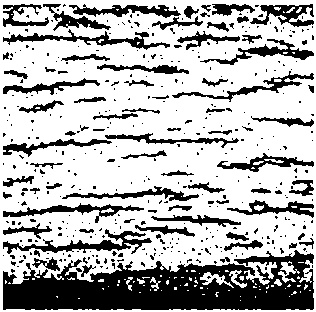
\includegraphics[width=0.4\textwidth]{Figures/not_blurred}\label{blur_notblur1}}
		\hfill
		\subfloat[The same micrograph with Gaussian blurring applied prior to filtering.]{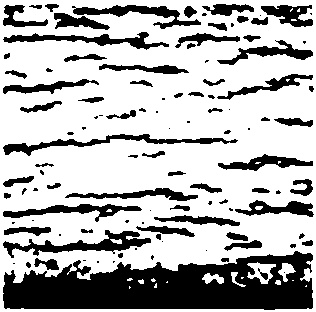
\includegraphics[width=0.4\textwidth]{Figures/blurred}\label{fig:blur_notblur2}}
		\caption{Comparison between identical micrographs both with and without the application of a Gaussian blur algorithm.}
		\label{fig:blur_notblur}
	\end{figure}
	\\
	\textbf{Gaussian blur theory}
	\\
	The Gaussian blur is typically used to smooth boundaries in an image where an immediate change in pixel intensity is observed compared to neighbouring pixels. The function typically employs a square matrix of values known as a \textit{kernel}. This kernel is 'superimposed' over the individual pixel values by an algorithm in a \textit{raster} pattern and alters their intensity accordingly.
	\[
	\frac{1}{16}
	\begin{bmatrix} 
		1 & 2 & 1 \\
		2 & 4 & 2\\
		1 & 2 & 1 \\
	\end{bmatrix}
	\longrightarrow
	\begin{bmatrix}
		0 & 10 & 170 & 220 & 130 & 30 & 10\\
		0 & 12 & 180 & 241 & 122 & 35 & 14\\
		2 & 13 & 176 & 237 & 134 & 43 & 7\\
		2 & 13 & 174 & 236 & 129 & 40 & 7\\
		1 & 11 & 159 & 224 & 132 & 31 & 5\\
		0 & 13 & 178 & 242 & 136 & 44 & 9\\
	\end{bmatrix}
	\]
	The above example depicts a 3$\times$3 Gaussian blur kernel, although larger dimensions such as 5$\times$5 may also be used. The binary image (represented here by a 7$\times$6 matrix of pixel intensities) is \textit{convoluted} through a specific matrix operation. This alters the pixel intensities of the filtered image as weighted by the values in the kernel. There are two possible ways to adjust the level to which the image is filtered; by increasing the dimensions of the kernel, which increases the range over which the intensities are averaged, or by adjusting the values in the kernel to provide a greater or letter degree of filtering. Each route provides its own merits and drawbacks.
	\\
	\\
	In the context of this report, both routes to alter the Gaussian mask were trialled. The method proposed by S. Khan involved using a module named \textit{OpenCV}, which is a cross-platform open source module that focuses on image processing techniques such as as greyscale to binary conversion, Gaussian and median blurring, filtering and thresholding. One approach of clarifying hydrides in the zirconium matrix was to initially blur and remove noise from the image followed by application of a pixel filter value as a method of binarising (i.e. identifying a threshold value between 0 and 255). The idea behind this approach was to allow a user to specify threshold and kernel blur values by calling a single function, \textit{image\_conv}, which would display a clear binarised image with applied Gaussian blur. A before and after histogram is also displayed to show how the previous 8-bit image is filtered to a binary image with 0 and 255 as integer values. Image blur was increased by altering the dimensions of the mask overlaying the micrograph image. This served to significantly reduce the noise observed in Figure \ref{blur_notblur1}, however the method relies primarily on an odd-integer input to specify square dimensions of 1,3,5..., etc. This can reduce the versatility of the technique as it limits control over the amount of blurring achieved for a specific region of pixels. 
	\\
	\\
	A. Hanson proposed a similar technique but instead utilising the \textit{Scikit image} or \textit{skimage} package. In this method the values within the Gaussian blur are adjusted through the use of altering the standard deviation from the mean used by the filter. Here, a larger specified value for $\sigma$ will produce a larger range of values within the kernel and generate a more intense blurring, whilst lower $\sigma$ values will generate higher \textit{relative} pixel intensities at the fringes of the kernel and thus reduce the level of blurring, see Figure \ref{fig:chu1gauss} (after binary thresholding). It was thought that this method proposed was more suited for the purpose of this study, as python code written in skimage allowed the gaussian blur $\sigma$ to be adjusted individually for each image.
	
	Using this approach, a function carries out the gaussian blur on an image array that has been read into python via \textit{skimage}, then the sigma values from the middle column of Table \ref{tab:imageprocessing} are specified in each case. There was also an additional input, \textit{truncation} value, which truncates the gaussian filter after the set amount of standard deviations. This was kept at a constant value of 3 throughout the study, as this was the default value recommended in skimage and also data within $3\sigma$'s accounts for 99.9\% of the data concerned. After this, images were ready for binary thresholding in the next function.
	\begin{figure}[h]
		\centering
		\subfloat[Image 'chu1' filtered using a Gaussian mask where $\sigma$=0.5]{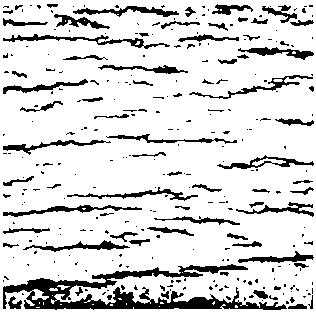
\includegraphics[width=0.4\textwidth]{Figures/chu1_s05_t04.jpg}\label{chu1_s05_t04}}
		\hfill
		\subfloat[Image 'chu1' filtered with $\sigma$=1.]{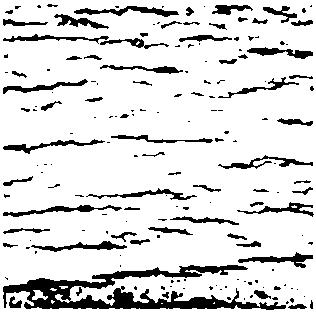
\includegraphics[width=0.4\textwidth]{Figures/chu1_s10_t04.jpg}\label{fig:chu1_s10_t04}}
		\caption{Post-processing of the same micrograph with differing values for $\sigma$. It is evident that higher values of $\sigma$ remove a larger quantity of noise between hydrides, but also result in aliasing of hydride boundaries and systematic removal of some regions.}
		\label{fig:chu1gauss}
	\end{figure}
	
	\subsection{Binary thresholding}
	Applying the same parameters in a Gaussian filter to different images tends to yield largely different results for the quantity of noise reduction in a range of images. In the sample image set provided for this investigation, many TEM micrographs exhibited a high degree of peripheral darkening, which leads to difficulties in applying an effective intensity threshold without suffering losses to the visible hydrides. As such, a threshold and standard deviation must be manually agreed upon for each image to ensure maximum hydride retention whilst eliminating a sufficient quantity of noise. This presents a significant limitation of the approach as large quantities of micrographs may become time-intensive to analyse. In addition, the systematic removal of small hydride regions may generate a significant source of error when cross-comparing images. Practically, this can cause an over- or underestimation of hydride quantity within a sample and difficulties may arise in subsequent connectivity analysis.
	\\ 
	\\
	For the sample set of images; \textit{chu1, chu2, chu3, chu7, chu11}, threshold and filter values (namely $=\sigma$) were agreed upon based on their perceived effectiveness as follows. Thresholding is a very simple operation and is applied with a simple python function that reads in the previously blurred image array, plots a respective histogram of it's pixel intensity values, and then applies the following operation, based on the specified threshold;
	\begin{center}
		In respective image array: $ value > threshold = true $
	\end{center}
	This sets any values in the image array greater than said threshold to true, numpy in python is then able to interpret this and convert this to an integer array of 1's and 0's which produces the binary images as displayed further on. In this case, a value of 1 is equal to white, when read in by skimage.
	\\
	\\
	Threshold values could be experimented with by simply running the code, viewing the histogram and going back to change the threshold to a more optimal value appropriately. Two sets of parameters were selected for each image conversion to highlight the effect of gaussian blurring and thresholding on the output images. This was done after some experimentation to find the appropriate range of values to find a satisfactory output image. 
	
	As such, the images filtered with the lower set of values are referred to as \textit{low-pass} (LP) and those filtered through higher values are denoted \textit{high-pass} (HP), see Table \ref{tab:imageprocessing}. It was decided to proceed to analysis with the low-pass binary images produced in an effort to reduce both excessive noise and excessive hydride omission.
	\\
	\begin{table}[ht]
	\begin{center}
	\begin{tabular}{ |c|c|c|c| } 
		\hline
		\multicolumn{4}{|c|}{Low-pass Images} \\
		\hline
		Image Reference & $\sigma$ (Gaussian blur) & Intensity Threshold Value & Gaussian Truncation Value \\
		\hline
		\textit{chu1} & 0.5 & 0.4 & 3 \\ 
		\textit{chu2} & 0.5 & 0.35 & 3 \\ 
		\textit{chu3} & 0.5 & 0.5 & 3 \\ 
		\textit{chu7} & 1.0 & 0.4 & 3 \\ 
		\textit{chu11} & 1.0 & 0.4 & 3 \\ 
		\hline
	\end{tabular}
	\\
	\begin{tabular}{ |c|c|c|c| } 
		\hline
		\multicolumn{4}{|c|}{High-pass Images} \\
		\hline
		Image Reference & $\sigma$ (Gaussian blur) & Intensity Threshold Value & Gaussian Truncation Value \\
		\hline
		\textit{chu1} & 1.0 & 0.5 & 3 \\ 
		\textit{chu2} & 1.0 & 0.4 & 3 \\ 
		\textit{chu3} & 1.0 & 0.4 & 3 \\ 
		\textit{chu7} & 1.0 & 0.6 & 3 \\ 
		\textit{chu11} & 1.0 & 0.5 & 3 \\ 
		\hline
	\end{tabular}
	\caption{Tested parameters gaussian blur $\sigma$ and binary threshold (see later sections) for the studied images using the \textit{scikit image} approach. This was split into low-pass and high-pass to investigate the effect of altering parameters.}
	\label{tab:imageprocessing}
	\end{center}
	\end{table}
	\\
These values generated the following pre-processed images shown in Figure \ref{fig:chu11LPHP}. It can be seen that the HP images have introduced much more noise and darkened areas, which warps the size of the hydrides.

%Is there an overall label for the combined figure? I dont know how to add it properly ~alex
	\begin{figure}[H]
		\centering
		\subfloat[\textit{chu1(LP)}: $\sigma$=0.5, T=0.4]{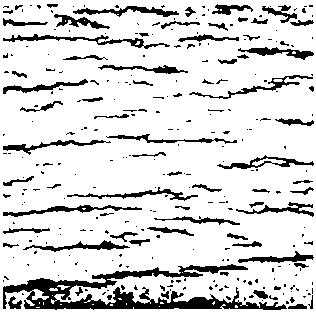
\includegraphics[width=0.4\textwidth]{Figures/chu1_binary3_sigma05_thres04.jpg}\label{chu1LP}}
		\hfill
		\subfloat[\textit{chu1(HP)}: $\sigma$=1.0, T=0.5]{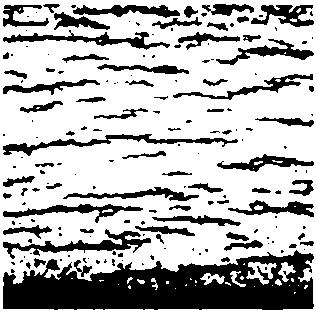
\includegraphics[width=0.4\textwidth]{Figures/chu1_binary1_sigma1_thres05.jpg}\label{chu1HP}}
		\label{fig:chu1LPHP}
		\subfloat[\textit{chu2(LP)}: $\sigma$=0.5, T=0.35]{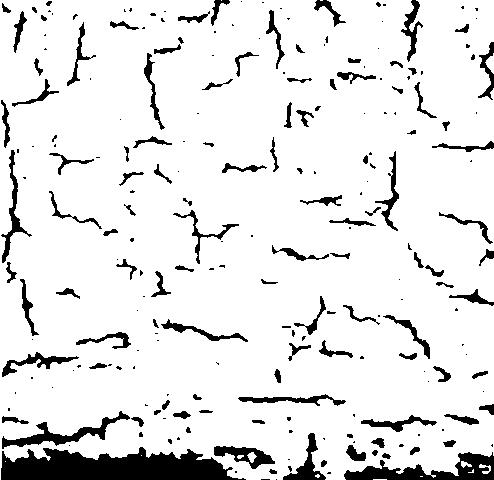
\includegraphics[width=0.4\textwidth]{Figures/chu2_binary3_sigma05_thres035.jpg}\label{chu2LP}}
		\hfill
		\subfloat[\textit{chu2(HP)}: $\sigma$=1.0, T=0.4]{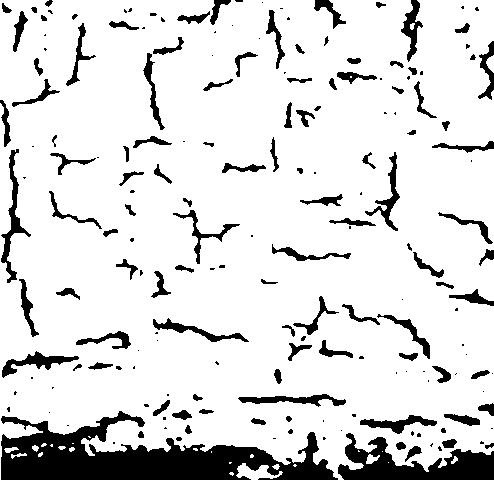
\includegraphics[width=0.4\textwidth]{Figures/chu2_binary1_sigma1_thres04.jpg}\label{chu2HP}}
		\label{fig:chu2LPHP}
		\subfloat[\textit{chu3(LP)}: $\sigma$=1.0, T=0.4]{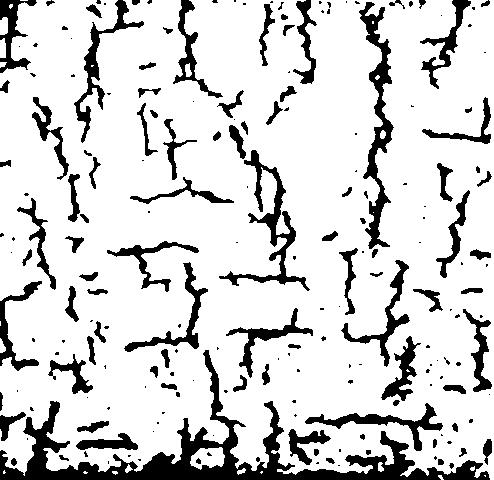
\includegraphics[width=0.4\textwidth]{Figures/chu3_binary1_sigma1_thres04.jpg}\label{chu3LP}}
		\hfill
		\subfloat[\textit{chu3(HP)}: $\sigma$=0.5, T=0.5]{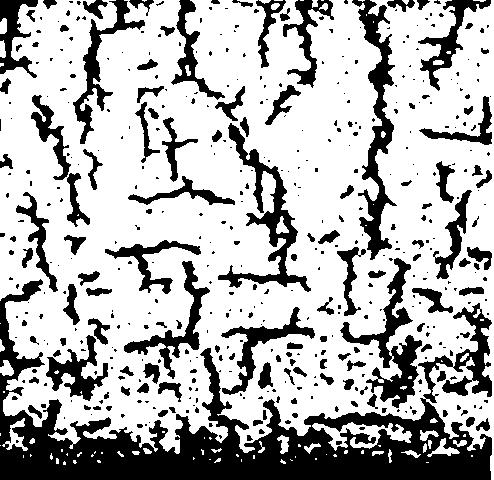
\includegraphics[width=0.4\textwidth]{Figures/chu3_binary1_sigma05_thres05.jpg}\label{chu3HP}}
		\label{fig:chu3LPHP}
	\end{figure}
	\begin{figure}[H]
		\centering
		\subfloat[\textit{chu7(LP)}: $\sigma$=1.0, T=0.4]{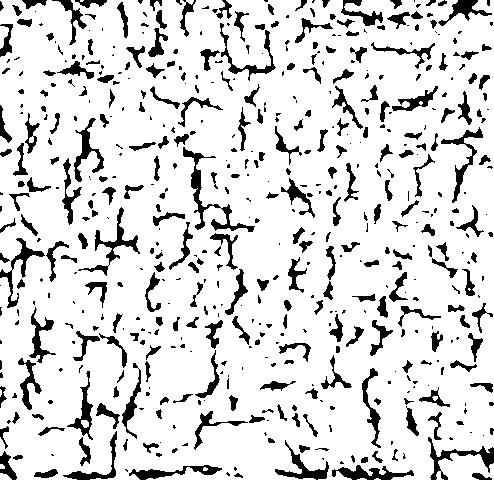
\includegraphics[width=0.4\textwidth]{Figures/chu7_binary1_sigma1_thres04.jpg}\label{chu7LP}}
		\hfill
		\subfloat[\textit{chu7(HP)}: $\sigma$=1.0, T=0.6]{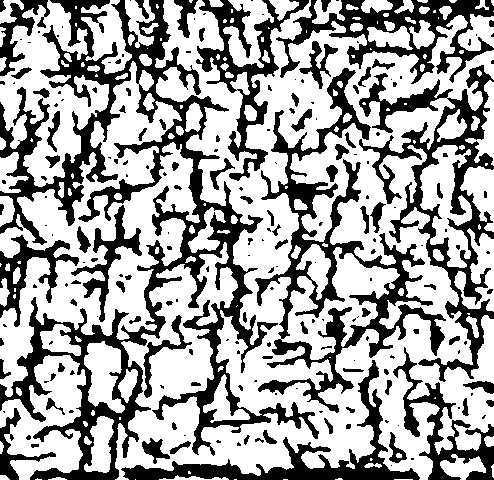
\includegraphics[width=0.4\textwidth]{Figures/chu7_binary2_sigma1_thres06.jpg}\label{chu7HP}}
		\label{fig:chu7LPHP}
		\centering
		\subfloat[\textit{chu11(LP)}: $\sigma$=1.0, T=0.4]{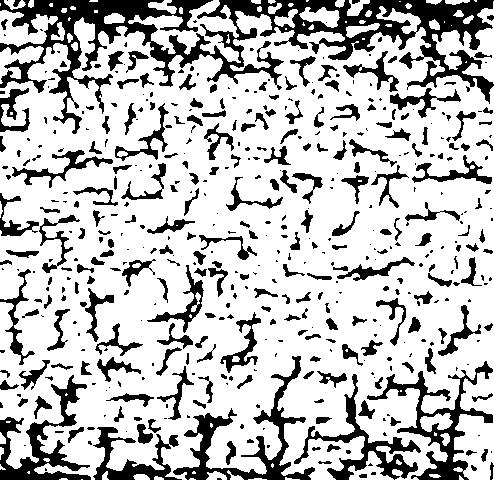
\includegraphics[width=0.4\textwidth]{Figures/chu11_binary1_sigma1_thres04.jpg}\label{chu11LP}}
		\hfill
		\subfloat[\textit{chu11(HP)}: $\sigma$=1.0, T=0.5]{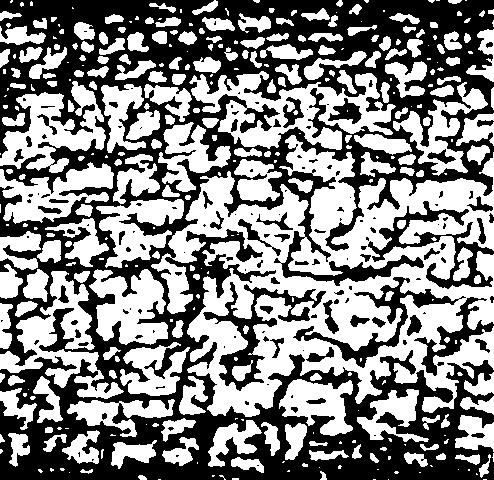
\includegraphics[width=0.4\textwidth]{Figures/chu11_binary3_sigma1_thres05.jpg}\label{chu11HP}}
		\label{fig:chu11LPHP}
		\caption{Pre-processed micrographs from the sample image set. Two images with differing threshold and $\sigma$ values are included for each micrograph.}
	\end{figure}

	\section{Initial Trial Methods to Assess Hydride Connectivity}
	Following pre-processing, techniques were trialled in an attempt to analyse the level of connectivity between regions of H\textsubscript{4}Zr in the micrographs \cite{Sharma2018}, \cite{Simon2021}, \cite{Sunil2020}.

	\subsection{Skeletonise function from Sci-kit Image}
	Skeletonisation was implemented as an initial approach for obtaining a simplified path for connected hydrides. This function would theoretically reduce the hydride map to a connected graph of thin lines (approximately one pixel in thickness). Using \textit{skimage.morphology}, the skeletonise() function was tested on image ‘chu1’. From the demo code produced, an initial reading of the file from the local directory was performed followed by specifying the image size. Using \textit{skblur} and \textit {skbinary}, ‘chu1’ was binarized and blurred to give the output as shown in Figure 4a. It is interesting to note that there were different variants to the skeletonise() function. One output (Zha84) initially takes the edges of an object (a hydride in this case) and iteratively removes pixels, stopping when the neighbouring pixel is black (where the intensity is zero) \cite{ScikitimageA}. As long as the image in Figure 4 (a) is inverted, the result is a series of single white pixel lines. Another output (Lee94) uses an 'octree' data structure which is more suitable for 3D images. Like Zha84, this algorithm also performs sweeping iterations over the image where pixels are continuously removed until the condition is satisfied where two iterations produce the same image and there is no change in the pixel count \cite{ScikitimageA}. Figure ~\ref{Zha84}  and Figure~\ref{Lee94} shows the results of Zha84 and Lee94 methods respectively, which were applied to the binarised ‘chu1’image from Figure 4a.
\\
	\begin{figure}[h]
		\centering
		\subfloat[Zha84 method of skeletonisation applied to 'chu1'.]{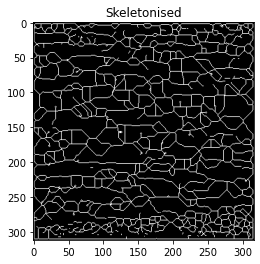
\includegraphics[width=0.4\textwidth]{./Figures/Skeletonised_Chu1}\label{Zha84}}
		\hfill
		\subfloat[Lee94 method of skeletonisation applied to 'chu1'.]{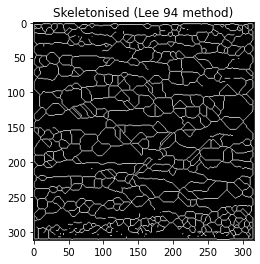
\includegraphics[width=0.4\textwidth]{./Figures/Skeletonised_Lee_Chu1}\label{Lee94_2}}
		\caption{Processing image 'chu1' with two skeletonisation methods. }
		\label{Skeletonise}
	\end{figure}
\\
	These results, however, are unsuitable for analysing connectivity as it appears that the matrix has been identified as the object rather that the hydrides themselves. Crucially, the skeletonise function does not provide actual data which can be applied to find suitable microstructural characteristics. Therefore, it was decided to assess an alternative characteristic of the microstructure to determine the hydride characteristics (discussed later). Finally, Figure~\ref{MedialAxis} below illustrates a representation of how \textit{medial\_axis} works by identifying the edges of the hydrides and then prints a skeleton (colour map=magma) \cite{Scikitimage}. In this case the skeleton is performed on the matrix rather than the hydride, this may be because of the initial ‘chu1’ binary image array, as these values are not inverted.
	\\
	\begin{figure}[h]
		\centering
		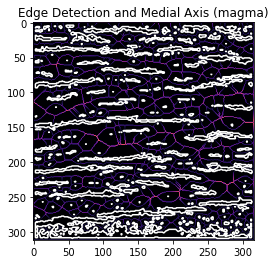
\includegraphics[width=2.5in]{Figures/Medial_Axis_Chu1} 
		\caption{Skeletonisation approach with medial axis pattern printed in a magma colour map, again applied to 'chu1'.}
		\label{MedialAxis}
	\end{figure}
	\\
	\subsection{Canny Edge Detection and the Hough Line Transform}
	
	The \textit{Hough Line Transform} relies on the detection of pixels within a series of lines superimposed onto a sample image. Rather than a typical first-order equation $y=mx+c$, the method defines these lines as the perpendicular normal to a line of angle $\theta$ from the top-left origin. Test text
	\\
	\\	
	It has been established that Hough transform is useful in detecting shapes using mathematical forms such as cartesian coordinates. For the case of straight lines, \textit{Hough space} can be used to identify the distance from the image origin to a line and the angle of the line relative to a specified axis. This description is for the OpenCV, \textit{cv2}, module which uses the ‘cv2.houghlines’ function. The main advantage of using Hough transform when put up against skeletonise is that it can return rho and theta values in a 2D array. Rho is the distance which is taken as positive if the line is above the origin and negative if the line is below the origin. Theta is the angle measured from the horizontal axis in the counter-clockwise direction. ‘Hough.transform’ uses the coordinate system (rho, theta) in a voting system \cite{OpenCV2013}. Here, a straight horizontal black line can be visualised in a white background image. If the start point of the line is at an initial value of (40, 90), ‘Hough.transform’ will detect this and begin searching the image to find matching the number of (40,90) cells. The maximum count for this cell would indicate that a line lies on this coordinate \cite{OpenCV2013}. When using the function, Canny edge detection was used to better visualise the hydrides. This function can also simply threshold and binarise an image, without allowing the user to change truncation or sigma values. After testing, the following results were given, as shown in Figure \_ (a) and (b). 
	\\	
	\begin{figure}[h]
		\centering
		\subfloat[Canny edge detection on image 'chu2']{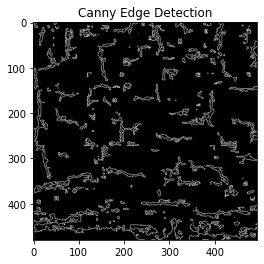
\includegraphics[width=0.4\textwidth]{./Figures/Canny_Edge_Detection}\label{Canny}}
		\hfill
		\subfloat[Attempted Hough transform on image 'chu2']{\includegraphics[width=0.4\textwidth]{./Figures/Hough_Transform_chu2}\label{Lee94}}
		\caption{Canny edge detection and hough.transform() used on image 'chu2' taken from Figure 4c. }
		\label{Skeletonise2}
	\end{figure}
	\\
\pagebreak
\\
\section{Radial Hydride Fraction to Assess Connectivity}
\subsection{Initial Approach using Hough Line Transform}

Due to difficulties in implementing a viable technique for determining the level of connectivity of hydrides within test micrographs, the focus of the project was adjusted to assist in determining the likelihood of through-wall cracking and subsequent mechanical failure of analysed zirconium samples. As previously highlighted, the rate of degradation of fuel cladding is dependent on the orientation of hydrides within the grains. However as observed many samples exhibit hydrides oriented both radially and circumferentially; a ratio is therefore needed to assess the contributions of the hydride orientations to the likelihood of failure by through-wall cracking. Known as the \textit{Radial Hydride Fraction} (RHF), this


%in one of my older notebooks, I wrote an explanation "connectivity testing" I think it was called - I'm not sure if it directly correlates to cracking
%Maybe we say that hydrides orientated radially are more likely of concern in cracking OR maybe you have already said that and I didn't get it :D

Initial approach, hough line transform over the whole image


\subsection{Refined Approach}
\textbf{Explain methodology that we use to obtain ACTUAL RHF - image slicing and the box!!!!}\\

The inputs for the \textit{hough\_measurebox} function are summarised in Table \ref{HoughmeasureboxInputs}. As there were many input parameters, it was decided that it would be best to have a standardised input for a reliable comparison between the resulting radial hydride fraction of images. As changing multiple inputs would make it impossible to make a proper comparison without extensive investigation. These inputs are based on documentation read in \cite{ScikitimageB}, which provides default and recommended values. More on the basis of choosing these is listed below:

\begin{itemize}
    \item \textit{Minimum distance between lines} - Adjusting this within the same order of magnitude seemed to have minimal effect, but it was not investigated in-depth.

    \item \textit{Minimum angle between lines} - This seemed suitable. It has a major effect on resulting output, but changing this would need further investigation.

    \item \textit{Fraction} - (Minimum peak intensity) It was found that 0.5 was too high, as this would eliminate objects less than 50\% size of the maximum detected object in said slice. This may reduce some key lines.

    \item \textit{Peak number} - This introduces large deviations in the detected lines, as all detected peaks will be plotted. 5 seemed appropriate
\end{itemize}

%WHY IS THIS TABLE MOVING?? :(
\begin{table}[h]
	\begin{center}
	\begin{tabular}{ |c|c|c| } 
		\hline
		\multicolumn{3}{|c|}{\textbf{hough\_measurebox Inputs}} \\
		\hline
		\textbf{Function Input} & \textbf{Value} & \textbf{Basis for Chosen Input} \\
		\hline
		\textit{Background value} & 1 & Always set to white. \\
		\hline
		\textit{Minimum distance between lines} & 5 & The default skimage value, seems suitable. \\ 
		\hline
		\textit{Minimum angle between lines} & 5 & The default in skimage, assumed to be degrees. \\
		\hline
		\textit{Fraction} & 0.3 & The default is 0.5 in skimage. \\ 
		\hline
		\textit{Peak number} & 5 & The default value is assumed maximum in skimage. \\ 
		\hline
	\end{tabular}
	\caption{Inputs for the slicing hough line transform function in python, used for the analysis of each image.}
	\label{HoughmeasureboxInputs}
	\end{center}
\end{table}

\subsection{Implementing Automatic Testing}
In order to learn how to implement automatic testing using GitHub and Python, and to check reliability of the analysis of the code in this study, automatic testing was implemented. This was done using the Python Application GitHub action in Git workflows, utilising the \textit{pytest} package. As it is difficult to automatically test the image processing steps of the study, it was thought to assess the the analysis of RHF as this is a quantity that can be somewhat predicted. So a methodology was proposed to produce a number of "test hydride" images which had a known radial hydride fraction, or in this case approximately estimated based on the previously explained criteria of RHF. Figures \ref{TestImages64} and \ref{TestImage300} below shows the test images created.

%is there a way to neaten out this hspace without a hfill ??
\begin{figure}[h]
		\begin{center}
		\subfloat[Test image 1, 64 by 64 pixels, with 3 radially orientated false hydrides]{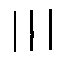
\includegraphics[width=0.2\textwidth]{./Figures/Test_1.jpg}
		\label{TestImage1}}
		\hspace{6pt} 
		\subfloat[Test image 2, 64 by 64 pixels, Test Image 1 rotated by 90 degrees]{
\includegraphics[width=0.2\textwidth]{./Figures/Test_2.jpg}
		\label{TestImage2}}
		\caption{The first test hydride images produced of 64 by 64 pixel size.}
		\label{TestImages64}
		\end{center}
	\end{figure}

\begin{figure}[h]
    \begin{center}
    
\includegraphics[width=2.0in]{Figures/Test_3.jpg} 
    \caption{Test image 3, 300 by 300 pixels, with a single circumferential hydride.}
    \label{TestImage300}
    \end{center}
\end{figure}

The test images were produced in ImageJ software, setting the background as white (a value of 255 when read into skimage) and the fake hydrides as black (0). The first 2 images were set to image size of 64 pixel squares, with approximately 40 pixel object lengths (these were drawn on with angles 90\degree and 0\degree respectively). The third image was created in the same manner, except its size was set to 300 by 300 pixels, as this is closer to the sample micrograph images assessed in the study. This image had only 1 fake hydride of 260 pixel length. These images should have Radial hydride fractions of 1.0, 0.0 and 0.0 respectively if the code functions as it should and detects only these singular objects in the hough transform.

Based on this, a testing procedure was proposed which sets a number of criteria that pytest would be able to test the images against using the \textit{assert} command. For \textbf{Test image 1}, a wholely radially orientated image, this cycled through:

\begin{center}
    Test 1: $assert\:RHF > 0.8$ \newline
    Test 2: $assert\:RHF > 0.9$ \newline
    Test 3: $assert\:RHF == 1.0$ \newline
\end{center}

For \textbf{Test images 2 and 3}, similar criteria were set but reversed as the fake hydrides were orientated in the circumferential direction, as follows:
\begin{center}
    Test 1: $assert\:RHF < 0.2$ \newline
    Test 2: $assert\:RHF < 0.1$ \newline
    Test 3: $assert\:RHF == 0.0$ \newline 
\end{center}

These criteria would allow users to see if a test image fell into the expected RHF range depending how it is orientated, and then finally it can be checked to see if the function is truly accurate by assessing whether RHF is equal to 1.0 or 0.0.  However before doing this the images must be pre-processed similarly to the micrographs analysed in the study, which means running them through \textit{skblur} and \textit{skbinary} in the test code. To minimise the effect that these may have, they were run with specified inputs shown in Table \ref{tab:TestImageTable}. A Gaussian blur sigma and binary threshold of 0 is used, to produce no blurring and to set any image objects to binary pixels.

\begin{table}[h]
    \centering
    \begin{tabular}{|c|c|}
    \hline
        \textbf{Function parameter} & \textbf{Test image input}  \\
        \hline
        $\sigma$ (Gaussian blur) & 0.0 \\
        \hline
        Gaussian Truncation Value & 3 \\
        \hline
        Intensity Threshold Value & 0 \\ 
    \hline
    \end{tabular}
    \caption{Test image pre-processing parameters used for \textit{skblur} and \textit{skbinary}.}
    \label{tab:TestImageTable}
\end{table}

After this, testing could be implemented with the criteria as explained above in each case. A separate test .py file was made for each test image, and then whenever the testing reposity was pushed or a pull request was created, the test workflow would run.

\section{Results and Discussion}
\subsection{Resulting Radial Hydride Fractions}
Results

influence of peak number on RHF - 1, 5, 10 - greater detect-ability of objects within images.

Noise as top \& bottom of image does influence results - larger objects are created and detected as being large hydrides.

\subsection{Automatic Testing Pytest Results}
The output of the tests produced by the Git workflow as summarised in Table \ref{TestResults}.

\begin{table}[h]
    \centering
    \begin{tabular}{|c|c|c|}
    \hline
        \textbf{Test Image} & \textbf{Tests Passed} & \textbf{Output RHF From Testing}  \\
        \hline
        1 & 3/3 & 1.0 \\
        \hline
        2 & 1/3 & 0.13 \\
        \hline
        3 & 2/3 & 0.01 \\
        \hline
    \end{tabular}
    \caption{The output of the automatic testing with pytest on GitHub using test images.}
    \label{TestResults}
\end{table}

It can be seen from the results, that only Test image 1 was able to pass all tests. Test images 2 and 3 failed some of the criteria. This is made obvious when looking at the output RHF in Table \ref{TestResults}. Test image 2 shows an unexpected result, and Test image 3 has some marginal error and is 1\% out from the expected value. This is not a major concern for Test image 3, as it is approximately correct (though the code does not recognise this), however for Test image 2 these is quite a high margin of error with RHF being approximately 13\% greater than expected. In order to verify what this may, the images were run through the python functions manually using inputs from Table \ref{tab:TestImageTable} to see the hough transform output. This is shown in Figure \ref{TestImagesProcessed} for Test images 2 and 3.

%I cant seem to get latex to detect these figures but they are in the right area?
\begin{figure}
    \centering
    \subfloat[Test image 2 processed]{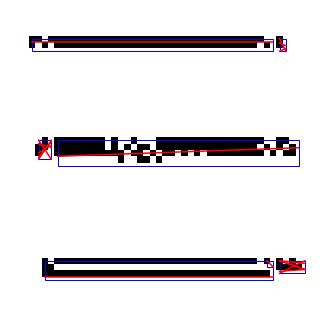
\includegraphics[width=0.4\textwidth]{Figures/test2_processsed.png}}
    \hfill
    \subfloat[Test image 3 processed]{
\includegraphics[width=0.4\textwidth]{Figures/test3_processsed.png}}
    \caption{Test images run through hough\_measurebox using default inputs, some noise is seen from the binary thresholding which highlights a problem.}
    \label{TestImagesProcessed}
\end{figure}

One of the image processing stages (likely the binary thresholding stage, as gaussian blurring was eliminated using $\sigma$=0) has generated some \textit{noise} or \textit{pixel artefacts} on the fake hydride objects in the images. This can be seen in both images, Figure \ref{TestImagesProcessed} a and b, of 64 and 300 square pixel size. However, it has had a larger effect on the smaller image, as any introduced small objects from noise or error will have greater effect. In Test image 2, there are 2 smaller objects which have been effectively broken off the main objects by the noise which leads to smaller hydrides which could be orientated in any direction according to the code. This could lead the hough transform to interpret these as being aligned perpendicular to the intended test hydride direction (circumferential), hence there is a deviation in the RHF leading to the error. In Test image 3, this has had a very slight effect due to the main object size dominating RHF, hence it has only deviated by ~1\%. 

These observed effects however do highlight a major problem in the image processing binary threshold stage or the nature of the test, which could be an effect of simple manual thresholding. In this case the threshold was set to 0, and as values of true black in hex code or RGB code (from ImageJ) are all 0's, this should have been interpreted as 0 in \textit{skblur} and \textit{skbinary} and the threshold applied on any non-black pixels. Here some pixels were obviously interpretted as greater than 0 despite they should be read as 0 values. This may have been an issue with the image production method using ImageJ drawing software, to verify this, Test Image 2 was read into \textit{skbinary} manually and the histogram was observed, it displayed that there was a small distribution of values around pixel intensity 0 and 255, not just the 2 polarised values. So ideally if the threshold was set properly, each object would be fully binarised and the automatic tests would have passed on each image. However, this may not be a good approach as the test images would have to be viewed, read in and analysed manually first to see what threshold and blurring parameters should be applied to "optimise" their condition for the hough line transform and RHF analysis tests. This partially eliminates the purpose of the automatic testing, and it may introduce some bias to the testing parameters. It is thought that it may be better to set up a test with default or expected parameters first, view the outcome and then attempt to learn and adjust code from there rather than the former. This however does highlight opportunities for future work in the area regarding the binary thresholding method and the automatic testing approach.



\section{Conclusions}
\subsection{On Hydride Structure Analysis}

\subsection{Recommendations}

\newpage
\bibliographystyle{IEEEtran}
\bibliography{References}

\newpage
\appendix
\section{: Making the code user friendly}
Small description on how functions were written to make the process easy for the user.

\end{document}
